\documentclass[a4paper]{article}
\usepackage[dutch]{babel}
%\usepackage{eurosym}
%\usepackage{hyperref}
%\usepackage{graphicx}
%\usepackage{amsmath}
%\usepackage{amssymb}
%\graphicspath{{./Images/}}
\usepackage{verslag}

\begin{document}

\section{Analyse oude systeem}
In dit hoofdstuk worden de mechanische aspecten en responsie van het oude mechanisme afgeleid en behandeld. Aan het einde van dit hoofdstuk worden conclusies getrokken over de sterke en zwakke punten van het huidige systeem.

\subsection{Algemene informatie}
(plaatje van opstelling met maten(SW)) \\
Zoals hierboven te zien is, bestaat de huidige rechtgeleiding uit twee verschillende bladveren met maten respectievelijk (lxbxh) ,van \textbf{()} die samen ervoor zorgen dat de rechtgeleiding met een bepaalde slag kan bewegen. Verder valt gelijk op te merken dat door het gebruik van twee bladveren het systeem overbepaald is.

Bij het gebruiken van twee bladveren treedt er shortening op, dit wil zeggen dat het blok bij een uitwijking niet op gelijke hoogte blijft zitten. Er zijn twee bladveren met een verschillende lengte dus voor elke bladveer is de shortening berekende aan de hand van,
\begin{equation}
y=\frac{-0.6x^2}{l}
\end{equation}
Als maximale uitwijking van het systeem is 7.5mm genomen, volgens figuur \ref{Shortening} blijkt dat het shortening effect dan 1.3mm is. Echter is voor de exacte volging van de VCM, alleen een translatie in de x-richting gewenst. Door shortening vindt echter ook een kleine beweging in de y-richting plaats. Om deze beweging zoveel mogelijk te neutraliseren zou er een constructie moeten komen die shortening tegen gaat. 
\begin{figure}[h]
\label{Shortening}
\centering
\setlength\figureheight{5cm}
\setlength\figurewidth{0.9\textwidth}
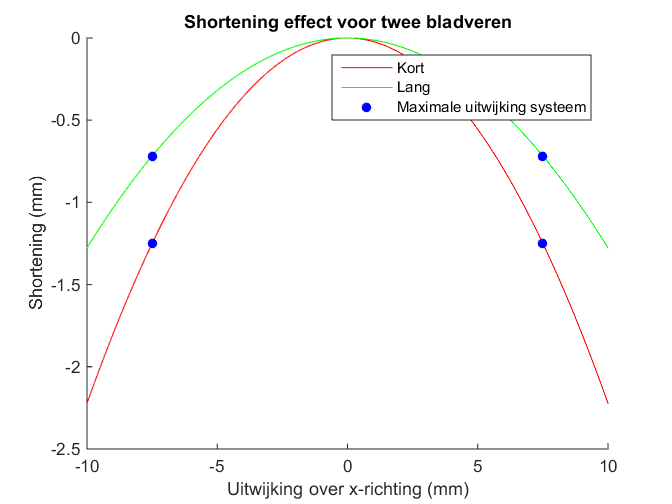
\includegraphics[width=0.75\textwidth]{Shortening.tikz}
\caption{Daling Blokje door Shortening}
\end{figure}

\subsection{Systeemresponsie}
Met behulp van een van de beschikbaar gestelde opstellingen (opstelling 12) is de stapresponsie \textbf{(afbeelding)} bepaald met behulp van een blokvormig signaal
\begin{figure}[h]
  \centering
    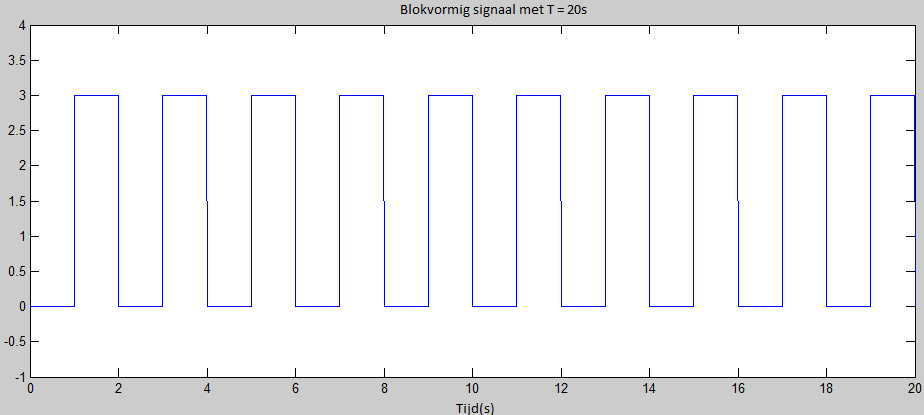
\includegraphics[width=0.55\textwidth]{Inputsignaal.png}
    \caption{Het gebruikte blokvormig signaal}
\end{figure}

\begin{figure}[h]
  \centering
    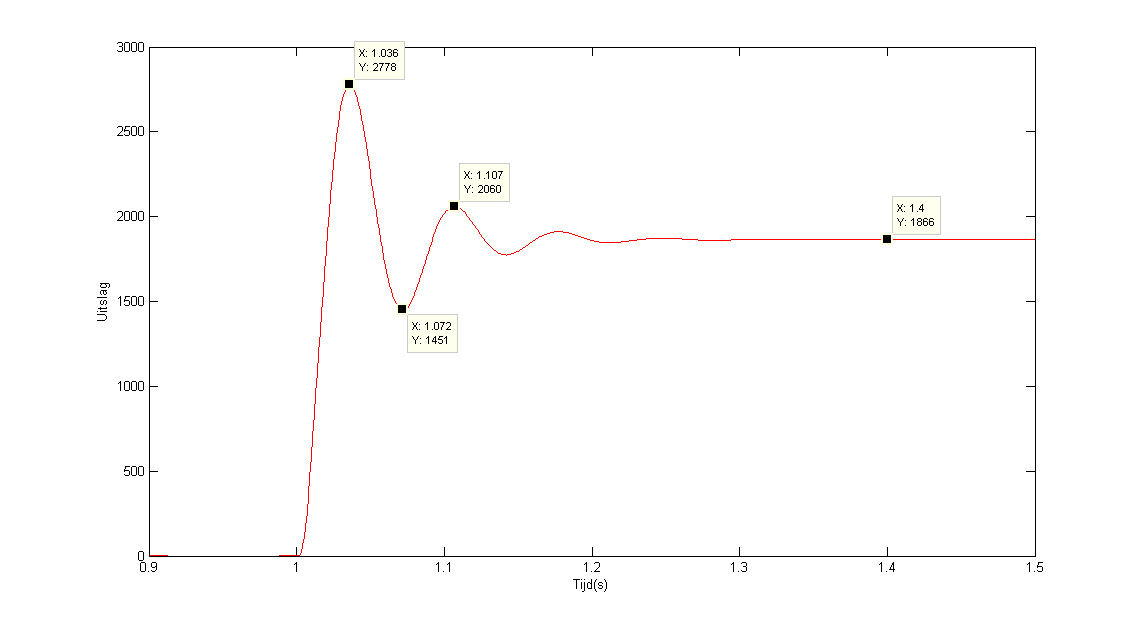
\includegraphics[width=0.95\textwidth]{Opstelling_12_stapresponsie.png}
    \caption{Representatieve stapresponsie met data-markers}
\end{figure}

Het bestaande systeem kan benaderd worden met een gedempt massa-veersysteem, De responsie van dit systeem kan vervolgens gemodeleerd worden met een tweede orde overdrachtsfunctie. 
\begin{equation}
G(s) = K * \frac{\omega_n^2}{s^2 + 2 \zeta \omega_n s + \omega_n^2}
\end{equation}
Met behulp van de overshoot en de peak-time die te bepalen zijn uit afbeelding \textbf{(Stapresponsie)} kunnen $\zeta$, $\omega_n$ en de versterking $K$ bepaalt worden.
\begin{equation}
\zeta = \frac{1}{\sqrt{1 + (\frac{\pi}{\ln(OS})^2}} \ \ \ with \ \ OS = \frac{x(t_p)}{x(\infty)} -1
\end{equation}
\begin{equation}
\omega_n = \frac{\pi}{t_p \sqrt{1 - \zeta^2}} \ \ derived \ from \ \ \omega_d = \frac{\pi}{t_p} \ \ and \ \ \omega_d = \omega_n \sqrt{1-\zeta^2}
\end{equation}
\begin{equation}
K = \frac{x_{response}(\infty)}{x_{signal}(\infty)}
\end{equation}
De waarden voor $K$, $\zeta$ en $\omega_n$ zijn dus gelijk aan: $ K = 622$, 
$\zeta = 0.223$ en $\omega_n = 89.5 \frac{rad}{s} = 14.2 \ Hz$.\\
De overdrachtsfunctie van dit systeem wordt dus gelijk aan:
\begin{equation}
G(s) = 622 * \frac{8013}{s^2 + 39.86 s + 8013}
\end{equation}
(plaatje) \\
Als afbeeldingen (stapresponsie en overdrachtres) met elkaar vergeleken worden word bevestigd dat de berekende overdrachtsfunctie een goede benadering is van dit systeem. 

\subsection{Mechanische constanten}

De mechanische constanten die bepaald moeten worden zijn de massa van het systeem, de dempingsconstante en de veerconstante. Gegeven is de eigenfrequentie,\\ 

\begin{equation}
\omega_n=\sqrt{\frac{k_{eq}}{m}}, \ \ \ \omega_n=14.2Hz
\label{Eigenfrequentie1}
\end{equation}

De veerconstante \ref{BDPP} kan uitgedrukt worden als,
\begin{equation}
k=\frac{Eht^3}{l^3}, \ \ \ k_{eq}=k_1+k_2
\label{Veerstijfheid} 
\end{equation} 
Dit geeft $k_1=864$$N/m$, $k_2=256$$N/m$, invullen in \ref{Eigenfrequentie1} geeft een massa van 140g. Voor de bewegingsvergelijking moet de dempingsconstante \ref{•} berekend worden aan de hand van,
\begin{equation}
2\zeta\omega_n=\frac{d}{m}
\end{equation} 
Dit geeft een totale dempingscoefficient van 5.6$Ns/m$.\\

\subsection{Eigenfrequenties}
Een van de belangrijkere systeemeigenschappen zijn de eigenfrequenties van het systeem. Het is wenselijk om de 1ste eigenfrequentie (van de ontworpen beweging) zo laag mogelijk te maken, terwijl de hogere eigenfrequenties zo hoog mogelijk gemaakt worden om ongewenste bewegingen te onderdrukken. Het huidige systeem is in Spacar gemodeleerd, en in figuren ()etc zijn de berekende eigenfrequenties te zien. Te zien valt dat de eerste eigenfrequentie overeenkomt met de eerder berekende, terwijl de hogere eigenfrequentie 130 resp 245 Herz zijn.
\subsection{Conclusies en aanbevelingen}
Een van de nadelen van het oude systeem is dat door het gebruik van twee bladveren het systeem overbepaald is wat zorgt voor ongewenste spanningen in de veren. \\ Tijdens experimenten zijn twee problemen duidelijk geworden, namelijk dat het systeem redelijk gevoelig is voor lompe studenten, waardoor de bladveren schuin komen te zitten, en het systeem klemt. Maar ook dat het systeem zeer gevoelig is invloeden van buitenaf (dit viel te zien in pieken als de opstellingstafel werd geraakt).  \\


\end{document}
